%%% DOCUMENT SETUP %%%
\documentclass[11pt,a4paper,onecolumn]{article}
\usepackage[english]{babel}

%%% LAYOUT %%%
\usepackage{fullpage}
\usepackage[parfill]{parskip}
\usepackage{multicol}
\usepackage{footnote}

%%% GRAPHICS %%%
\usepackage{graphicx}
\usepackage{color}
\usepackage{graphics}
\usepackage{rotating}
\usepackage{subfig}
\usepackage{amsmath}
\usepackage{amssymb}
\usepackage{amscd}
\usepackage{xfrac}
\usepackage{float}
\usepackage{dsfont}

%%% FONT %%%
\usepackage{ifxetex}
\ifxetex
  \usepackage{fontspec}
    \setmainfont{Linux Libertine O}
  \usepackage{xunicode}
  \usepackage{microtype}
\else
  \usepackage[T1]{fontenc}
  \usepackage[latin1]{inputenc}
  \usepackage{times}
  \usepackage{microtype}
\fi

%%% Coding %%%
\usepackage{listings}
\usepackage{pseudocode}

%%% TITLE PAGE %%%
\author{Jeroen Hofman (10194754)  \\[15pt] University of Amsterdam (\textsc{UvA})}

\title{Scientific Computing\\
  Assignments \\
		}

\begin{document}
\maketitle
\captionsetup{width=0.8\textwidth}
\lstset{language=Python,breaklines=true,backgroundcolor=\color{white},frame=single}
\thispagestyle{empty}
\graphicspath{{/home/jhofman/Desktop/SC/assignment2/}{/home/jhofman/Desktop/SC/assignment3/}{/home/jhofman/Desktop/SC/assignment4/}}

%%% TABLE OF CONTENTS %%%
\newpage
\tableofcontents
\newpage

\section{Assignment 1: Matrix-Vector Multiplication}

\subsection{Introduction}
The first part of this report will be different from the subsequent parts, because the assignment given is rather small and does not have much theory behind it. We will describe briefly the algorithm used for matrix-vector multiplication with MPI in the Methods section, results will be given in the Results section, followed by a small conclusion and discussion in the section Conclusion.

\subsection{Method}
We implement a small program which, given a matrix size of $N$x$N$ and a number of processes $p$, executes in parallel matrix-vector multiplication. The code is available in \texttt{SC-10194754/assignment1/mult.c}. The program can be compiled by using \texttt{make} in the \texttt{assignment1} directory and shall be run as follows:\\
\begin{center}
  \texttt{mpiexec -n <number of processes> mult.o <matrix size>}
\end{center}
In the code we begin by starting a timer after we have assigned every process a rank. Then every process computes which part of the matrix it should use for the multiplication, i.e. which chunk size it will get. We will use division in the row order here, which is easy to implement and also works best concerning cache locality (though this beyond the scope of this course). The method used is an integer division of the matrix size $N$ divided by the number of threads $p$. Then the leftover given by $N - p*\sfrac{N}{p}$ is distributed among the processes, since this is always a number between 0 and $p$, some processes will receive one row extra while others will receive none, the chunk size is referred to as $nrows$. Also an offset value is computed for every chunk, i.e. which row of the original matrix is the zero row of the matrix of a particular process.

After the workload is divided we create 3 dynamically allocated arrays on each process, one for the matrix of size $nrows * N$, one for the vector which is multiplied of size $N$ and one for the result vector, also of size $N$. We initiate the vector elements by the index of the element, but only perform this initialization on the rows which correspond to the chunk (the assigned rows) of that particular process. We initiate the matrix elements by the index of the row of the complete matrix.

Furthermore we allocate two more arrays of size $p$, with a value in each element equal to the length of the chunk for the process rank corresponding to that element and another array giving the offset per rank. Since we want every process to have the whole vector and not just the rows corresponding to its chunk we have to use \texttt{MPI\_Allgatherv} to send the complete vector to every process. Since the exchanged size is not necessarily constant (since not all the chunks have to have the same size), \texttt{MPI\_Allgather} does not work properly. \texttt{MPI\_Allgatherv} needs an array with lengths of the data to send and an array for the offsets, so it knows where to place them, hence the need for the two extra dynamically allocated arrays as defined above. The gathering acts as a barrier, i.e. all processes will not go beyond this point before they all have a complete vector.

After the gathering is complete, every process computes a part of the result vector, by multiplying one of the rows of its matrix by the (now entirely filled) vector. After all processes have completed this they send the computed part of the result vector (so not the whole vector) with \texttt{MPI\_Isend} to the process with rank 0, which receives the data with \texttt{MPI\_Irecv} and then calls \texttt{MPI\_Waitall} to suspend until it has received all messages. When this process has received all messages it calls the timer again and computes the total elapsed time.

\subsection{Results}
\subsubsection{Performance}
We measured the total execution time $T_p$ with $p$ the number of processes, the relative speedup $T_1/T_p$ and the relative efficiency $S_p/p$ for matrix sizes 1000, 5000 and 10000 and 1..8 processes. The measurements are performed on LISA nodes with 8 cores and 1 process per node. Since we are interested in the best performance we have repeated each measurement 3 times and we report the best results in terms of performance. The results are given in Table \ref{tab:mult} below.

\begin{table}[H]
  \centering
  \begin{tabular}{l | c | c | c}
    \# Processes & Execution Time & Relative Speedup & Relative Efficiency \\
    \hline
    \multicolumn{4}{c}{$n = 1000$} \\
    \hline
    1 & 0.002113 & 1 & 1 \\ 
    2 & 0.001109 & 1.91 & 0.95 \\
    3 & 0.000761 & 2.78 & 0.93 \\
    4 & 0.000574 & 3.68 & 0.92 \\
    5 & 0.000451 & 4.68 & 0.94 \\
    6 & 0.000420 & 5.03 & 0.84 \\
    7 & 0.000380 & 5.53 & 0.79 \\
    8 & 0.000381 & 5.52 & 0.69 \\
    \hline
    \multicolumn{4}{c}{$n = 5000$} \\
    \hline
    1 & 0.053582 & 1 & 1 \\
    2 & 0.026988 & 1.98 & 0.99 \\
    3 & 0.018176 & 2.95 & 0.98 \\
    4 & 0.014183 & 3.78 & 0.94 \\
    5 & 0.010843 & 4.94 & 0.99 \\
    6 & 0.011818 & 4.53 & 0.76 \\
    7 & 0.007837 & 6.84 & 0.98 \\ 
    8 & 0.007900 & 6.78 & 0.85 \\
    \hline
    \multicolumn{4}{c}{$n = 10000$} \\
    \hline
    1 & 0.200818 & 1 & 1 \\ 
    2 & 0.107516 & 1.87 & 0.93 \\ 
    3 & 0.072043 & 2.78 & 0.93 \\
    4 & 0.053852 & 3.72 & 0.93 \\
    5 & 0.045421 & 4.42 & 0.88 \\
    6 & 0.038699 & 5.19 & 0.86 \\
    7 & 0.030677 & 6.55 & 0.93 \\
    8 & 0.032948 & 6.09 & 0.76 \\
  \end{tabular}
  \caption{Execution time, relative speedup and relative efficiency as a function of matrix size and number of processes.}
  \label{tab:mult}
\end{table}

From the table above we observe that there is a significant speedup when increasing the number of processes. The speedup is equally large for smaller matrix sizes as for larger matrix sizes, this indicates that the overhead is the dominant factor in the algorithm described above. Indeed, the gathering used to obtain the vector and the receiving and sending are relatively expense compared to the simple inner product. In tests with MPI performed before (not for this course) the efficiency usually gets better for larger matrices, since the actual computation (e.g. doing the inner product) increases faster in terms of computation time than the overhead, here it is however not the case. It is a matter of preference whether or not to include the initialization in the execution time, based on the examples given for this course, we choose to include the initialization into the time measurement. Speedups will be better if this part is not included in the time measurement. 

For a matrix of size 1000x1000 we find a maximum speedup of a factor 6.55, which corresponds to an efficiency of 93\%. For all matrix sizes the difference in performance in 7 and 8 cores is very small, this is caused by a remark also given in the documentation on LISA: using 7 cores on an 8-core machine leaves one core for scheduling and other (OS) tasks, and hence this might increase performance, and indeed we see the effect that adding an extra core by going to 8 cores does not give a performance increase. Most likely the speedup gained by adding an extra core and the slowdown by having to switch to OS tasks on already occupied cores balance each other out, leading to a similar performance between 7 and 8 cores. 

\subsubsection{Evaluating complexity}
We will now attempt to give a very rough evaluation of the time complexity of the algorithm as described in the section Methods. We will also attempt to link this to the results given above, i.e. finding this overhead term that dominates the speedup by parallelising the inner product. We can calculate the execution time per process as follows:

\begin{equation}
  T_p = \frac{N}{p} * N * \tau_{\text{calc}} + 2\tau_{\text{setup}} + 2\frac{N}{p}\tau_{\text{exchange}}
\end{equation}
 
The matrix-vector multiplication has $\frac{N}{p}*N$ terms for each process. The \texttt{MPI\_Allgatherv} sets up communication between each process (so to $p-1$ other processes for every process, but done in parallel) and it then sends its own data $p-1$ times and receives from others also $p-1$ times. We assume here that sending and receiving can be done in parallel, and sending/receiving to/from multiple processes can also be done in parallel. Then every thread opens communication with the master thread, and sends $\frac{N}{p}$ to the master thread. This explains the factor two. Notice again that we assume that communication to multiple processes is as fast as communication to one single other thread.

Judging from this equation the dominant factor is the matrix vector multiplication if $N$ is large, and hence this problem has a complexity of roughly $\sfrac{N^2}{p}$. However, there is substantial overhead in the gathering function, as well as in the sending and receiving at the end. Indeed when the time measurement is solely placed around the matrix vector multiplication we get almost perfect speedup (not given in the table). So most likely the terms $\tau_{\text{setup}}$ and $\tau_{\text{exchange}}$ are much larger than $\tau_{\text{calc}}$, such that they dominate the time it costs to do the actual matrix-vector multiplication.

We can also theoretically analyze other decompositions. One such decomposition would be to divide the matrix in columns strips instead of rows strips. The amount of computation would be the same, $\sfrac{N^2}{p}$, but a process would only need its own part of the vector (since only the first $\sfrac{N}{p}$ columns of the matrix are multiplied with the first $\sfrac{N}{p}$ rows of the matrix, which the process already has in our setup). However this multiplication will produce a vector of length $N$ per process, and so a whole vector has to be sent to the master process and then the master process has to add it up, this gives for the complexity:

\begin{equation}
  T_p = \frac{N}{p} * N * \tau_{\text{calc}} + \tau_{\text{setup}} + n*\tau_{\text{exchange}}
\end{equation}

So the difference with the previous decomposition is less setup time, but more exchange, it will depend on the number of processors and $\tau_{\text{exchange}}$ and $\tau_{\text{setup}}$ which one is faster (we assume the adding up of the result vectors is very fast).

Another possible decomposition is a block-wise decomposition which is essentially a combination of both. The size of such a block is roughly $\sfrac{N}{\sqrt{p}}$. A process does not need the whole vector, but it needs a portion equal to $\sfrac{N}{\sqrt{p}}$, but since the process of sending the vector is assumed to be done concurrently, and if we assume that a given process at least needs the data from one other process (which will be the case for $p \geq 4$), the communication term does not change. The outcome however is a vector of length $\sfrac{N}{\sqrt{p}}$, which has to be sent to the master thread, which then has to combine the vectors and add them up (which we assume is done fast). We then obtain the following formula:

\begin{equation}
  T_p = \frac{N}{p} * N * \tau_{\text{calc}} + 2\tau_{\text{setup}} + (\sfrac{N}{p} + \sfrac{N}{\sqrt{p}})*\tau_{\text{exchange}}
\end{equation}

which is smaller than the column-wise decomposition if $p$ is very large and $\tau_{\text{setup}}$ is small. It is however always larger than the row-wise decomposition, since $\sfrac{N}{p} + \sfrac{N}{\sqrt{p}} > 2\sfrac{N}{p}$.

\subsection{Conclusion}

We developed an MPI program for matrix-vector multiplication and found a significant speedup for increasing number of processes. However, the speedup does not scale with the number of processes, caused by the enormous overhead created by \texttt{MPI\_Allgatherv} and the sending and receiving at the end of the calculation. The matrix-vector multiplication is too simple and fast as an operation to counter these overhead costs, at least in the matrix sizes considered here.

\newpage

\section{Assignment 2: The Vibrating String}

\subsection{Introduction}
In this assignment we look at the behavior of a vibrating string, which either starts in a sine-position or in a plucked position. After describing the algorithm we look at the behavior of the string, and measure the speedup and efficiency with MPI. We also look at some stability issues.

\subsection{Theory}
We study the wave equation in one dimension, given by:

\begin{equation}
  \label{eq:wave}
  \frac{\partial^2 \Phi}{\partial t^2} = c^2 \frac{\partial^2 \Phi}{\partial x^2}
\end{equation}

We can discretize this equation by setting $t = n \delta t$ and $x = l \delta x$. We can use a Taylor expansion around $c(x,t\pm \delta t)$, giving the following result:

\begin{equation}
  \Phi(x,t\pm \delta t) = \Phi(x,t) \pm \frac{\partial \Phi(x,t)}{\partial t} + \sfrac{1}{2}\delta t^2 \frac{\partial^2 \Phi(x,t)}{\partial t^2} + \mathcal{O}{\partial t^3}
\end{equation}

Adding these two equations and rewriting gives:

\begin{equation}
  \frac{\partial^2 \Phi}{\partial t^2} = \frac{\Phi(x,t+\partial t) - 2\Phi(x,t) + \Phi(x,t-\partial t)}{\partial t^2}
\end{equation}

Repeating this for the second derivative of $x$ gives (using exactly the same method):

\begin{equation}
    \frac{\partial^2 \Phi}{\partial x^2} = \frac{\Phi(x+\partial x,t) - 2\Phi(x,t) + \Phi(x-\partial x,t)}{\partial x^2}
\end{equation}

If we substitute these two expression in equation \ref{eq:wave}, we obtain:

\begin{equation}
  \label{eq:disc}
  \Phi(x,t+\partial t) = 2\Phi(x,t) - \Phi(x,t-\partial t) + \tau^2(\Phi(x+\partial x,t) - 2\Phi(x,t) + \Phi(x-\partial x,t))
\end{equation}

which is our final finite difference equation with $\tau = \frac{c\delta t}{\delta x}$. If we create a grid with distances between points of $\delta x$ and time steps $\delta t$ we see that increasing the time step (i.e. doing one iteration) is a function of the current values of the neighboring points, the current value of the point itself, and the value of the point one iteration before. By adjusting the value of $\tau$ different types of behavior can be observed, we will come back to this later.

\subsection{Method}
We implement a program which, given some parameters as input, calculates the movement of a vibrating string. The code is available in \texttt{SC-10194754/assignment2/wave.c}. The program can be compiled by using \texttt{make} in the \texttt{assignment2} directory and shall be run as follows:\\
\begin{center}
  \texttt{mpiexec -n <number of processes> wave.0 {-s <number of sine functions on string> || -p <plucked position>} -n <number of grid points> -d <timestep> -t <runtime> -v <visualize frequency>}
\end{center}
We will now describe the algorithm that is used in \texttt{wave.c}. In the main-body of the code we start by initializing MPI with \texttt{MPI\_Init}. We then parse the parameters given in the command line to the process with rank 0 and store them in a struct \texttt{parms}, which is then sent to all other MPI processes. This is all done by the function \texttt{getparms()} given by the \texttt{apr} library which is provided. Since we are given the C-code of this function (instead of just the \texttt{apr} library), there is not much use in writing our own function for this as we have access to the source.

After parsing the parameters and sending them off to every process, we initialize the topology on the processes. In this case we choose a ring topology, implying an infinite string, which is created by calling \texttt{MPI\_Cart\_create}. The processes then all obtain a rank and they can find out their neighbors rank with respect to the topology by calling \texttt{MPI\_Cart\_shift}. After this setup is completed they enter a barrier, to ensure that parsing the parameters and creation of the topology has finished on all threads. We then proceed by letting process 0 start the time measurement.

The next step is computing the data decomposition, which is done in a similar way as in the last assignment. We divide the number of grid points (which is an input parameter) among the processes such that the maximum difference of workload between processes is 1 grid point. We allocate an array of this workload size plus two extra points (\emph{nvalues}) to every process, since we will need this extra points for computing the values at the boundaries (they are the copies of the boundary points of the neighboring processes). Every process gets three arrays allocated of this size, one for the current iteration values (\texttt{curval}), one for the old values (\texttt{oldval}), and one for the new iteration to be computed (\texttt{newval}). 

After the allocation is completed the visualization is called by all processes if enabled in the command line options. We then initialize the string, either in the plucked position or in the sine position. In the sine position we compute the position of the grid point on the string (the string has length 1) and then take the sine of that position multiplied by <number of periods> * $2\pi \ $ <number of grid points> and store this in the \texttt{curval} array. We assume here continuous boundary conditions, i.e. the outer left element of the string 0 is a copy of the \emph{nvalues} - 2 element, and the outer right element \emph{nvalues} - 1 is a copy of element 1. 

For the plucked position however we have to do a little bit more work, given the position of the plucked position (given as input parameter) we calculate the slope of the lines left of this point and right of this point. Then given a grid point we calculate its position $x$ on the string (again the string has length 1) which is between 0 and 1. If the position is to the left of the plucked position our value is $x$ * <slope\_left>, otherwise it is $1 + (x - $ <plucked position>) * <slope\_right>. We need to take special care of processes which have rank 0 or rank <processes - 1> because for their outer left (0) and outer right (\emph{nvalues} - 1) points this does not hold, they are assumed to be mirrors of element \emph{nvalues} - 2 and element 1 respectively. After initialization these values are copied to \texttt{oldval}.

We now proceed with the main iteration loop, where the number of iterations is given by the \texttt{ceil} of <runtime> / <timestep>. We now proceed with the loop where first every step the visualization is called if the frequency coincides with the iteration number. We then call a function \texttt{compute()} which does all the important work. When the processes enter this function they first compute $\tau^2$ as given in the Theory section. Then they iterate over all their grid points (not the copied points!) and calculate the next iteration using equation \ref{eq:disc} from the previous section. After the iteration is complete the pointers to the arrays are swapped, so \texttt{curval} becomes \texttt{oldval} and \texttt{newval} becomes \texttt{curval}. \texttt{newval} gets the address of \texttt{oldval} to ensure there are no memory leaks. This method of pointer swapping is much faster than using \texttt{memcpy} for instance, since it does not actually do anything except swapping some pointers, which is very fast. However one has to be careful by assuming static buffers, sine this is not the case anymore. In my specific setup however this is not a problem. 

After switching the arrays each process sends it own boundary points 1 and \emph{nvalues} - 2 and receives copied points at position 0 and \emph{nvalues} - 1 from another process using \texttt{MPI\_Isend} and \texttt{MPI\_Irecv}. The processes suspend in a \texttt{MPI\_Waitall} waiting for all communication to be completed. After the communication every process has the correct copied points corresponding to the new iteration which has just been computed. The processes than continue with the next iteration step. Instead of the above communication method one could also use \texttt{MPI\_Sendrecv}, however this does almost exactly the same, when testing the two functions no difference in performance was found. For the sake of readability we will use the first method of \texttt{MPI\_Isend} and \texttt{MPI\_Irecv}. 

After the maximum number of iterations is reached we do one final visualization and end the time measurement. The program is cleaned up by deallocating the arrays and calling \texttt{MPI\_Finalize}.

In the method described above we explicitly parallelize the string in the spatial instead of the temporal domain, which would also have been an option. However, implementation of parallelization in the temporal domain is much more difficult, since the dependencies are much larger between subsequent time steps than they are between different spatial positions of the string. Spatial decomposition only involves exchanging the boundary points as described above, however the state at time $t$ depends on the state at time $t-1$, which depends on itself on the state at time $t-2$ etc., so there is a fixed order in which these calculations have to done, namely in chronological order. This is however not the case for the spatial domain, as the calculation of a point $x+1$ at a given time is not dependent on the new value of $x$ at that time, only on the old values, so this is much easier to parallelize.

\subsection{Results}
\subsubsection{Tests}
We perform a series of tests with the following parameters to check the correct working of our program:
\begin{itemize}
\item 
  Number of grid points on string: 100, so $\delta x = 0.01$.
\item
  $\tau$: 0.5, if we pick $c$ = 1 then this implies $\delta t = 0.005$. This is assumed to be stable, as we will see later. 
\item
  Runtime: 10
\item
  Report frequency: 1, we will filter out suitable values for $t$ later.
\item
  Method: either a sine with period 1 or a plucked string at position 0.3.
\end{itemize}

We run the program using the above parameters and visualize the string using \texttt{Mathematica}. The experiments are performed on a HP netbook with 2 cores, since we are interested in behavior, not performance. Figure \ref{fig:sine} below gives the time evolution of the vibrating string with the sine function, figure \ref{fig:plucked} below gives the time evolution of the plucked string.

\begin{figure}[H]
  \centering
  \subfloat{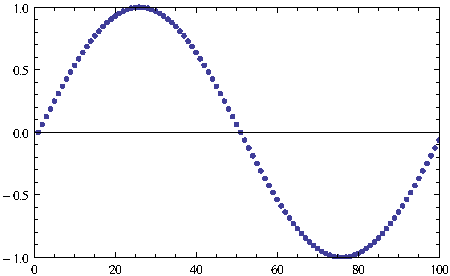
\includegraphics[width=0.3\textwidth]{string1.pdf}}
  \subfloat{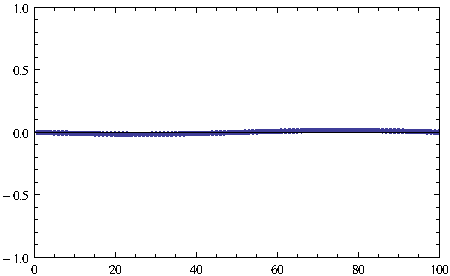
\includegraphics[width=0.3\textwidth]{string2.pdf}}
  \subfloat{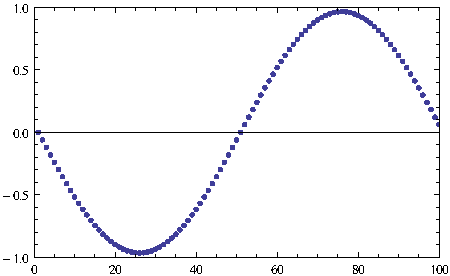
\includegraphics[width=0.3\textwidth]{string3.pdf}}
  \\
  \subfloat{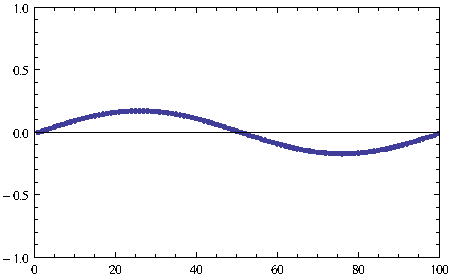
\includegraphics[width=0.3\textwidth]{string4.pdf}}
  \subfloat{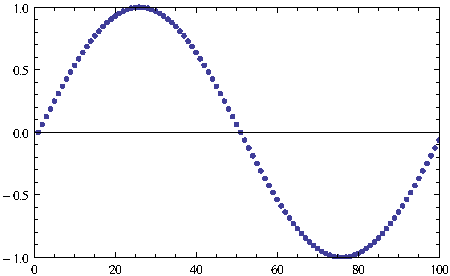
\includegraphics[width=0.3\textwidth]{string5.pdf}}
  \caption{Five different snapshots for the vibrating string with the sine function, for $t = 0$, $t = 0.25$, $t = 0.45$, $t = 0.78$ and $t = 1.00$.}
  \label{fig:sine}
\end{figure}

\begin{figure}[H]
  \centering
  \subfloat{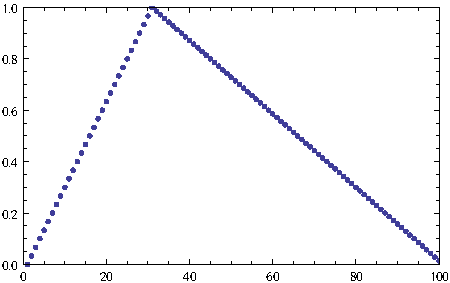
\includegraphics[width=0.3\textwidth]{string6.pdf}}
  \subfloat{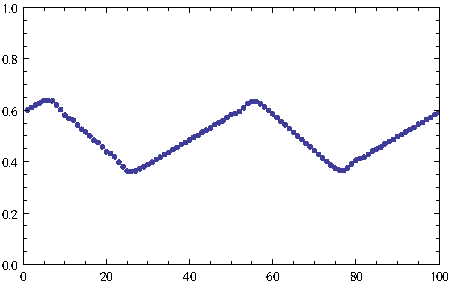
\includegraphics[width=0.3\textwidth]{string7.pdf}}
  \subfloat{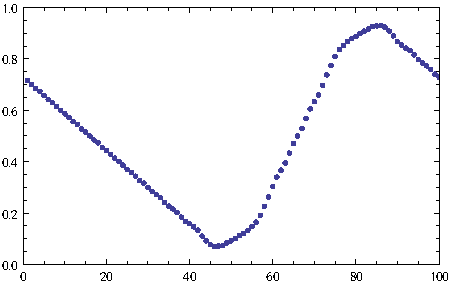
\includegraphics[width=0.3\textwidth]{string8.pdf}}
  \\
  \subfloat{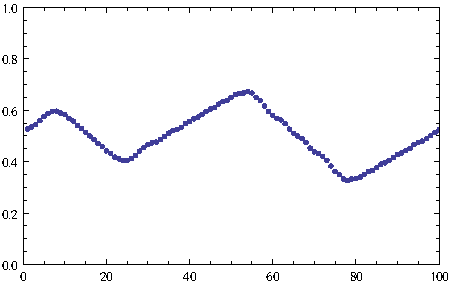
\includegraphics[width=0.3\textwidth]{string9.pdf}}
  \subfloat{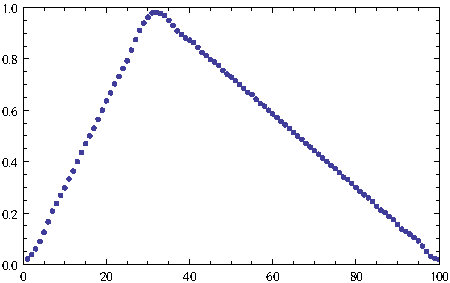
\includegraphics[width=0.3\textwidth]{string10.pdf}}
  \caption{Five different snapshots for the vibrating string with the plucked function, for $t = 0$, $t = 0.25$, $t = 0.45$, $t = 0.78$ and $t = 1.00$.}
  \label{fig:plucked}
\end{figure}

Figure \ref{fig:sine} shows that the vibrating string with a sine function behaves as expected. Starting with the original sine function (left,top) the string contracts first into a straight line (middle,top) and then expands again in the other direction (right,top), to contract again (left,bottom) and finally expand again (right,bottom), completing the cycle.

For the plucked string we can observe similar behavior, however the behavior of this is a little less intuitive (since this is not a real physical system). We start with an initial plucked string (left,top) and if we imagine an equilibrium line around 0.5, everything above this line starts moving down, while everything below starts moving upwards, the moving is faster as the particular part of the string is farther away from equilibrium. This results in the next figure (middle,top), if we continue this we end up with a shifted maximum and minimum compared to the initial situation (right, top). Finally, the string starts moving towards the center again (left,bottom) to end up in the original state (right,bottom). Notice that these figures are not taken exactly at all special moments (i.e. fully stretched or contracted), but slightly off these moments to show some intermediate behavior.

The somewhat strange behavior of the plucked string can be explained by this particular implementation where no fixed boundary points are used, since if fixed points were used, the maximum would have shifted continuously to a minimum and back. However, letting the string not be constrained gives a more complex and interesting behavior, especially when the plucked position is not 0.5, when the string would be symmetrical.

It also should be noted that these strings do not represent physical strings, because their length is not fixed (and replacing strings by elastic springs gives a whole new set of problems) as well as the energetically unfavorable state of the plucked string, where the string makes an angle of 90 degrees, which causes great resistance by internal forces in the string. The angle of 90 degree would certainly not occur again when the string has been released which is however the case in our model.

\subsubsection{Stability}
In finite difference approximations such as the wave equation stability of the solution is very important. If the solution is not stable it will produce incorrect results after a finite amount of time. In the particular case of the wave equation it can be shown that the system is stable only when $0 \leq \tau \leq 1$, hence we choose $\tau = 0.5$ in the previous section to show the behavior of the vibrating string. To show the instability of the system we will perform the same computation as in the previous section, with the difference of taking $\tau = 1.1$ and hence with $c = 1$ and $\delta x = 0.01$ this implies taking $\delta t = 0.011$. Figure \ref{fig:chaos} below shows snapshots at the system at the same times used in the previous section.

\begin{figure}[H]
  \centering
  \subfloat{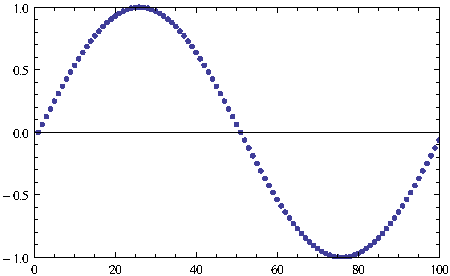
\includegraphics[width=0.3\textwidth]{string11.pdf}}
  \subfloat{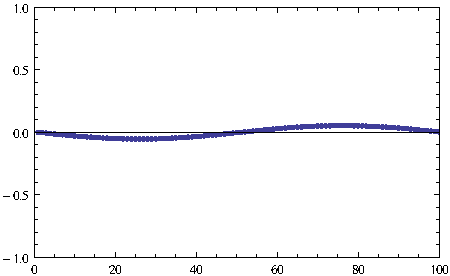
\includegraphics[width=0.3\textwidth]{string12.pdf}}
  \subfloat{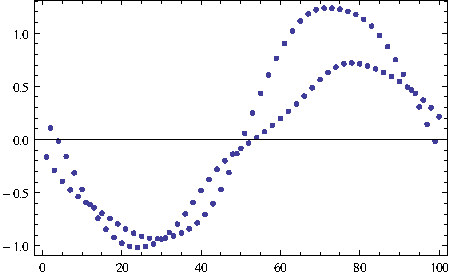
\includegraphics[width=0.3\textwidth]{string13.pdf}}
  \\
  \subfloat{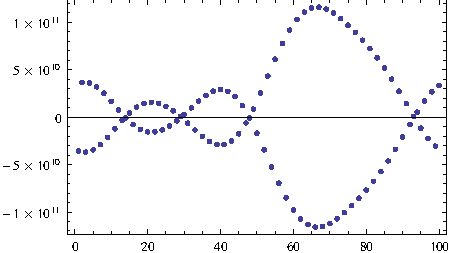
\includegraphics[width=0.3\textwidth]{string14.pdf}}
  \subfloat{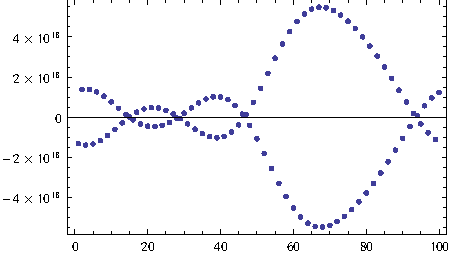
\includegraphics[width=0.3\textwidth]{string15.pdf}}
  \caption{Five different snapshots for the vibrating string with the sine function, for $t = 0$, $t = 0.25$, $t = 0.45$, $t = 0.78$ and $t = 1.00$.}
  \label{fig:chaos}
\end{figure}

Clearly the system is unstable, since it starts off just like the stable version, a full sine (left,top) followed by a contraction (middle,top). But after this the points start diverting and the whole system explodes, leading to values as high as $10^{18}$ already for $t = 1.00$. To examine the behavior of the system as a function of $\delta t$ we can do a series of measurements on the system and check when the onset of unstable behavior starts (this is done by eye, but it is still a good approximation).

\begin{table}[H]
  \centering
  \begin{tabular}{l | l}
    $\delta t$ & Onset of instability (time steps) \\
    \hline
    0.01 & - (stable) \\
    0.011 &  0.407 (step 37)\\
    0.02 & 0.26 (step 13)\\
    0.05 & 0.40 (step 8)\\
    0.10 & 0.40 (step 4)\\
  \end{tabular}
  \caption{Onset of instability as a function of $\delta t$.}
\end{table}

The table shows that although the absolute time at which the instability occurs is more or less the same, the number of steps decreases for increasing $\delta t$. This makes sense because if $\delta t$ increases, the accuracy with which the system is computed decreases, and decreasing accuracy leads to increasing errors and these errors will perturbate through the system. The larger the error, the faster it will show up in the system because of this perturbation, and the faster the system will collapse.

\subsubsection{Scalability}

We measure the scalability of the system by using the following parameters:
\begin{itemize}
\item 
  Number of processes: 1..8 (one process per node)
\item
  Number of grid points: $10^4, 10^5, 10^6$
\item
  Report frequency: 0 (no reporting)
\item
  Method: 1 sine
\item
  $\tau$ = 0.5, giving $\delta t = \tau$ * 1/<number of grid points>
\item
  $t$ = $\delta t * 10^4$
\end{itemize}

In this way we ensure that the number of time steps is constant, as well as $\tau$ (and hence we have a stable system). We perform the measurements on 8 LISA nodes with one process per node. Table \ref{tab:wave} gives the results of these measurements:

\begin{table}[H]
  \centering
  \begin{tabular}{l | c | c | c}
    \# Processes & Execution Time & Relative Speedup & Relative Efficiency \\
    \hline
    \multicolumn{4}{c}{$N = 10^4$} \\
    \hline
    1 & 0.258262 & 1 & 1 \\ 
    2 & 0.189669 & 1.36 & 0.68 \\
    3 & 0.192079 & 1.34 & 0.44 \\
    4 & 0.169017 & 1.53 & 0.38 \\
    5 & 0.148169 & 1.74 & 0.35 \\
    6 & 0.137375 & 1.88 & 0.31 \\
    7 & 0.136125 & 1.90 & 0.27 \\
    8 & 0.123946 & 2.08 & 0.26 \\
    \hline
    \multicolumn{4}{c}{$N = 10^5$} \\
    \hline
    1 & 2.520613 & 1 & 1 \\
    2 & 1.320721 & 1.90 & 0.80 \\
    3 & 1.135706 & 2.21 & 0.74 \\
    4 & 0.866701 & 2.90 & 0.73 \\
    5 & 0.700948 & 3.60 & 0.72 \\
    6 & 0.672724 & 3.76 & 0.63 \\
    7 & 0.594000 & 4.27 & 0.61 \\ 
    8 & 0.526992 & 4.75 & 0.59 \\
    \hline
    \multicolumn{4}{c}{$N = 10^6$} \\
    \hline
    1 & 47.486079 & 1 & 1 \\ 
    2 & 18.971037 & 2.63 & 1.315 \\ 
    3 & 10.173441 & 4.67 & 1.56 \\
    4 & 6.705000 & 7.08 & 1.77 \\
    5 & 5.394558 & 8.80 & 1.76 \\
    6 & 4.515187 & 10.52 & 1.75 \\
    7 & 3.987887 & 11.91 & 1.70 \\
    8 & 3.458008 & 13.73 & 1.72 \\
  \end{tabular}
  \caption{Execution time, relative speedup and relative efficiency as a function of grid points and number of processes.}
  \label{tab:wave}
\end{table}

From Table \ref{tab:wave} we can derive some results. First we see that for small number of grid points ($10^4$) the speedup is not very large, only a factor 2.08 for 8 cores compared to 1 core. The efficiency is a meager 0.26. This low efficiency is caused by a large overhead which is dominant over the speedup achieved by chopping the string into equally sized pieces. The speedup gets better when we go to $10^5$ points, with an efficiency of 0.59, corresponding to a speedup of 4.75 for 8 cores compared to 1 core.

The best result however is obtained for $10^6$ points, with a speedup which is super linear (i.e. scales better than linear with the number of cores). We achieve a speedup of a factor 13.73 for 8 cores, which has an efficiency of 1.72. The only reason super linear speedup is achieved is by looking at the cache size. The problem as stated above has a memory usage which comes mainly from the three matrices which are involved (the old, new and current ones). The size in memory of these matrices is 3 * 8 * $10^6$, since they are made of doubles which have size 8. This totals to around 24MB in size. The cache size on LISA is 6MB, so if we use 4 processes or more the matrices should fit in the cache, significantly speeding up the execution, since a memory load is very expensive compared to a load from cache. Indeed from the results we see the efficiency increasing until the number of processes is 4, after that it is more or less stable, because adding extra processes does not increase the amount of the matrices that fits in the cache, since everything is already being stored there. The reason that there still is a super linear speedup from 1 to 2 cores for example, while in both cases the matrices do not fit in cache completely, is that a larger part of the matrices fits in the cache in the case of 2 processes compared to 1.

Lastly the better speedup for larger grids is enhanced because of the ratio of time steps compared to grid points. If this ratio is large (i.e. many time steps, few grid points), communication will play a significant role since this scales linear with the number of time steps, whereas the actual computation time for the grid depends on the number of grid points. As $N$ increases, this ratio becomes smaller, as we keep the number of time steps fixed to $10^4$ and hence the time spent on communication becomes smaller, this also explains why speedups are much better for larger $N$ than for small $N$.

\subsection{Conclusion}
We implemented a vibrating string using MPI. We found correct behavior as far as the physical behavior of the vibrating string is concerned. We found unstable regions in which the solution diverges quickly for increasing time. We also tested the scalability and found poor scalability for small grid sizes, increasing to super linear scalability for large grid sizes, caused by storage of matrices in the cache and a relatively smaller communication overhead.

\newpage

\section{Assignment 3: Diffusion on a Cylinder}
\subsection{Introduction}
In this assignment we model diffusion on a cylinder in two dimensions. We first look at the theory and the complexity at the problem, then we look at some results of the program and finally we look at the scalability of the problem.

\subsection{Theory}
We study the diffusion equation in two dimensions, given by:

\begin{equation}
  \frac{\partial c}{\partial t} = D (\frac{\partial^2 c}{\partial x^2} + \frac{\partial^2 c}{\partial x^2})
\end{equation}

where $D$ is the diffusion coefficient. We can again discretize this equation, following the procedure from the last assignment, which gives (the derivation is not given here):

\begin{equation}
  \label{eq:diff}
  c_{i,j}^{k+1} = c_{i,j}^k + \frac{\delta t D}{\delta x^2}(c_{i,j+1}^k + c_{i,j-1}^k + c_{i+1,j}^k + c_{i-1,j}^k - 4 c_{i,j}^k)
\end{equation}

It can be shown that this scheme is stable when $\sfrac{4 \delta t D}{\delta x^2} \leq 1$, which restricts the choice of $\delta x$ and $\delta t$. We see from the finite difference equation that the value of a grid point at the next iteration is only dependent on the value at the current iteration, unlike the discretization in the previous assignment, in which the previous iteration was also needed.

We further assume the following set of boundary and initial conditions ($1 \geq x \geq 0$,$1 \geq y \geq 0$,$t > 0$) :

\begin{align}
  &c(x,y=1,t) = 1 \; \text{and} \; c(x,y=0,t) = 0 \; \text{source and sink} \nonumber \\
  &c(x,y,t=0) = 0 \; \text{for all x and y > 0}
\end{align}

Furthermore we have continuous boundary conditions in the $x$ direction so $(x=0,y,t) = (x=1,y,t)$, making it a cylinder. With this set of equations the solution can be computed, however this is non-trivial to do, therefore we will not do that in this report. It can however be shown that for large $t$, $c(x,y,t) \rightarrow y$, which we will test in the Results section.

\subsubsection{Domain decomposition}

There are many ways in which the grid on which the computation is performed can be decomposed. We will consider two types of decompositions: row-decomposition and block-decomposition. In the case of the former the matrix is subdivided into chunks, each consisting of a number of adjacent rows roughly equal to the number of rows divided by the number of processes. In the latter case the matrix is divided into chunks, each consisting of a number of adjacent rows and columns (so not the entire rows) roughly equal to the square root of the number of processes. We can make the following analysis in the case of a row-decomposition:

\begin{align}
  \label{eq:row}
  T_{p} &= \frac{N^2}{p} \tau_{\text{calc}} + \frac{2N}{p}\tau_{\text{copy}} + \tau_{\text{comm}} \\ \nonumber
  &= \frac{N^2}{p} \tau_{\text{calc}} + \frac{2N}{p}\tau_{\text{copy}} + 2(\tau_{\text{setup}} + N\tau_{\text{exchange}}) 
\end{align}

where the size of the matrix is $N$x$N$. The execution time for $p$ processes $T_p$, is equal to the number of grid points that is assigned to each process, $\sfrac{N^2}{p}$ times the time it takes to do one calculation $\tau_{\text{calc}}$. We add to this the copying $\tau_{\text{copy}}$ of the first and last column per process to be able to mimic the continuous boundary conditions, as will be described in the next section. For the communication we need to exchange the first and last row assigned to every process to be sent to the neighboring processes, the first row to the left neighbor and the last row to the right neighbor. For this we need to set-up communication with two other processes taking time $\tau_{\text{setup}}$ and then we need to exchange 1 row, hence $N$ points taking time $\tau_{\text{exchange}}$, with the other processes. Every process also has to receive rows from the neighbor, but we assume this can be done concurrently with the sending of the rows, hence it will cost no extra time. Note that this analysis assumes every process has two neighboring processes, this is not the case for the first process and the last process.

For the block-decomposition we can make the following analysis:

\begin{align}
  T_P = \frac{N^2}{p}\tau_{\text{calc}} + 4(\frac{N}{\sqrt{p}}\tau_{\text{exchange}} + \tau_{\text{setup}})
\end{align}

Where the first term is similar to the row-decomposition. Every process now has to exchange roughly $\sfrac{N}{\sqrt{p}}$ points with 4 other processes, provided the process is entirely surrounded by other processes. There are however in the block-decomposition much more special cases, because when a process is at the top or bottom of the matrix it does not exchange to 4 but to 3 processes only. When it is at the left or right of the matrix it has to copy one side, but since it has to copy from another process (unlike the row-decomposition) the above formula still approximately holds.

We can make a comparison between these two methods by assuming that the setup time $\tau_{\text{setup}}$ is negligible, as well as the copying time $\tau_{\text{copy}}$, since the copying is performed on one process (so shared memory) and hence assumed to be much faster exchange between different memories. By this assumptions we see that block-decomposition is favorable when:

\begin{equation}
  \frac{4N}{\sqrt{p}} > 2N \rightarrow p > 4
\end{equation}

We will use only row-decomposition in the algorithm described in the next section for simplicity. We expect that for large matrices the execution time will scale linearly with the number of processes, since the dominant term for large $N$ will be $\frac{N^2}{p}\tau_{\text{calc}}$.

\subsection{Method}

We implement some code which, give some parameters as input, calculates the diffusion of some substance with the initial concentrations as described above over a cylindrical area. The code is available in \texttt{SC-10194754/assignment3/diff.c}. The program can be compiled by using \texttt{make} in the \texttt{assignment3} directory and shall be run as follows:

\begin{center}
  \texttt{mpiexec -n <number of processes> diff.o -n <matrix size of nxn> -d <timestep> -t <runtime> -v <visualize frequency (0 is none)>}
\end{center}

We will now describe the algorithm that is used in \texttt{diff.c}. We start the main body of the code by initializing MPI with \texttt{MPI\_Init} and parsing and sending all the command line parameters to the other processes using the \texttt{getparms} function available in the \texttt{apr} library, as in the previous assignment. Then we proceed by setting up the topology of the processes, which in this case is, like in the vibrating string assignment, a ring topology but without the exchange between the first and the last process, so it is a line topology. We determine the neighbors of every process by using \texttt{MPI\_Cart\_shift}, which gives the neighbors above and below the current process. 

After passing a barrier the first process starts the timer for our performance measurements. The data decomposition is then computed. Every process receives a number of rows which is roughly equal to the size of the matrix $N$, given by the command line argument, divided by the number of processes. The difference cannot be more than one row between processes, as we have implemented before in the vibrating string. Every process then allocates two arrays, one for the current values and one for the new values, where the arrays have a size equal to the matrix size $N$ plus two (for the extra columns on both sides to implement continuous boundary conditions) times the number of rows assigned to that process plus two, to store the neighboring rows from the other processes needed for the finite difference computation. Note that we use a peculiar structure for these arrays (\texttt{double (* NAME)[N][M] = (double (*)[N][M]) malloc(N*M*sizeof(double))}), since they are two-dimensional, but cast here in a form which makes them 1-dimensional in allocation, which speeds up the code due to cache locality.

We then do two more things for initialization: we link two global void arrays to the arrays just created (because the arrays cannot be passed easily to a function) and we initialize the arrays to 0, with the exception of the first row, which is set to 1, i.e. the initial condition as described in the Theory section. The first row, which is set to 1, is not actually part of the $N$x$N$ matrix, it is the extra top row from the first process. This translates to a situation where one side of the cylinder is in contact with some large system where the concentration is constant 1. We apply the same for the extra bottom row of the last process, which is constant 0, setting up the source-drain system.

We now enter the loop which iterates over the matrix. The loop first calls the visualize function if the current iteration is a multiple of the frequency given as command line argument. The function visualize is not taken from the \texttt{apr} library, since the function from the library only works properly for the vibrating string, but instead there is a \texttt{visualize} function defined above the main body of the code. It writes the local matrices to a file with name \texttt{data.i <current iteration> p <process>}. The files can be manually joined by using the \texttt{cat} command in Linux.

We now enter the heart of the code, namely the part where the actual computation is done. We define $D = \sfrac{\delta t}{\delta x^2}$ and make local copies of the two arrays, which are stored in the global variables (via linkage). This might seem expensive, but it is a simple pointer assignment, so no copying is performed. Then the finite difference equation \ref{eq:diff} is applied first to the first and last row of every matrix (not counting the 'extra' rows!). The processes then proceed by copying the values from the first column to the extra column on the right and the values from the last column to the extra column on the left. This is only done for the four values in total, two per row that has already been calculated. Since both rows which are neighboring another process are computed, the processes can start sending/receiving these rows to/from other processes to store it in the extra rows at the top and bottom of the matrices. We only initialize sending these rows by calling \texttt{MPI\_Isend} and \texttt{MPI\_Irecv}, but do not require the messaging to finish yet. While the messages are being sent the processes continue with calculating the rest of the new matrix by equation \ref{eq:diff} and after that the values from the first column are being copied to the extra row on the right and the last column to the extra row on the left. This method of splitting the calculation up to ensure early exchange of messages is much faster than first computing the entire new matrix and then start sending/receiving, since the sending/receiving and doing a computation can be done concurrently if the memory is not fully occupied.

After the new matrix is computed the processes wait for all communication to be complete with \texttt{MPI\_Wait}, which hopefully has been completed already while the processes were computing the inner part of the matrix. After the exchange of messages is completed the matrix pointers are swapped (again saving time by not copying) and an iteration is complete. 

After all iterations are completed a final visualization is done (if given by the command line argument) and finally the first process calculates the elapsed time. Then the arrays are properly deallocated and \texttt{MPI\_Finalize} is called.

\subsection{Results}
\subsubsection{Tests}
We first test the program on correctness using two properties described in the Theory section. First we look if the solution is independent of the $x$ direction, since all values in the $x$ direction are equal if $t \rightarrow \infty$ according to the theory. Secondly we look if the values are similar to the analytical values. Given a grid of length 1 and a matrix size of $N$ we find that $\delta x$, the distance between two grid points, is $\sfrac{1}{\delta x}$. We will take $D = 1.0$ to ensure stability, which leads to an expression for $\delta t = \delta x^2$. We performed measurements with $N = 100$ on 2 processors, giving $\delta x = 0.01$ and $\delta t = 10^{-4}$. Figure \ref{fig:diff} shows the concentration for $t = 0.001$ (top left), $t = 0.01$ (top right), $t = 0.1$ (bottom left) and $t = 1.0$ (bottom right).

\begin{figure}[H]
  \centering
  \subfloat{
\includegraphics[width=0.4\textwidth]{t0001.pdf}}
  \subfloat{
\includegraphics[width=0.4\textwidth]{t001.pdf}}
  \\
  \subfloat{
\includegraphics[width=0.4\textwidth]{t01.pdf}}
  \subfloat{
\includegraphics[width=0.4\textwidth]{t1.pdf}}
  \caption{Snapshots of diffusion on the cylinder for $t = 0.001$ (top left), $t = 0.01$ (top right), $t = 0.1$ (bottom left) and $t = 1.0$ (bottom right).}
  \label{fig:diff}
\end{figure}

Initially the concentration is zero everywhere except for the extra row at the top, then the diffusion starts and in the last picture there is more or less a constant gradient between the bottom and top of the matrix. Also the solution is clearly not dependent on the $x$ position, which was one of the validation points of the model.

We can also take one slice along the $y$ axis and plot the concentration as a function of $y$, see Figure \ref{fig:lin} below. We can compare this with the analytical values obtained from the analytical solution (the solid lines). We see that the solution as found by the finite difference is close to the analytical solution. Indeed we see that when time increases the concentration approaches the asymptote $c(x,y,t) = y$. We can conclude from these comparison that our model indeed shows the correct behavior.

\begin{figure}[H]
  \centering
  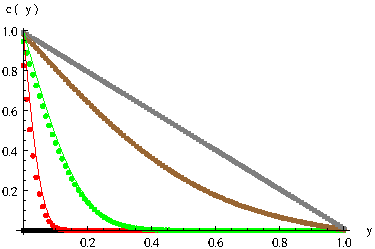
\includegraphics[width=0.7\textwidth]{linearity.pdf}
  \caption{The concentration as a function of $y$ for $t = 0.001$ (red), $t = 0.01$ (green), $t = 0.1$ (brown) and $t = 1$ (gray). The solid lines are the analytical solutions.}
  \label{fig:lin}
\end{figure}

\subsubsection{Scalability}

Like in the previous assignments, we can measure the scalability of this model. In line with the other assignments we measure the scalability of the whole program, not just on the iterations. We will do more extensive testing, namely for $N = 2^5 .. 2^{10}$ and $p = 1 .. 8, 16$. We balance $\delta t$ such that $D = 0.5$ in each case and we set the reporting frequency to 0. The results for the measurements (every measurement is repeated three times and the best value is reported) are given in Table \ref{tab:diff} below:

\begin{table}[H]
  \centering
  \begin{tabular}{l | c | c | c | c | c | c}
    \# Procs & Exec. Time & Rel. Speedup & Rel. Efficiency & Exec. Time & Rel. Speedup & Rel. Efficiency\\
    \hline
    \multicolumn{1}{c}{} & \multicolumn{3}{c}{$N = 32$} & \multicolumn{3}{c}{$N = 64$} \\
    \hline
    1 & 0.051747 & 1 & 1 & 0.147552 & 1 & 1\\ 
    2 & 0.096327 & 0.53 & 0.26 & 0.148239 & 0.99 & 0.50\\
    3 & 0.108142 & 0.48 & 0.16 & 0.177281 & 0.83 & 0.28\\
    4 & 0.110988 & 0.47 & 0.12 & 0.194024 & 0.76 & 0.19\\
    5 & 0.104232 & 0.50 & 0.10 & 0.123710 & 1.19 & 0.24\\
    6 & 0.099684 & 0.52 & 0.09 & 0.150131 & 0.98 & 0.16\\
    7 & 0.185417 & 0.28 & 0.04 & 0.119800 & 1.23 & 0.18\\
    8 & 0.108401 & 0.48 & 0.06 & 0.123191 & 1.20 & 0.15\\
    16 & 0.128551 & 0.40 & 0.03 & 0.129484 & 1.14 & 0.07\\
    \hline
    \multicolumn{1}{c}{} & \multicolumn{3}{c}{$N = 128$} & \multicolumn{3}{c}{$N = 256$} \\
    \hline
    1 & 0.499414 & 1 & 1 & 1.792005 & 1 & 1\\
    2 & 0.297742 & 1.51 & 0.76 & 1.096307 & 1.63 & 0.82\\
    3 & 0.312598 & 2.21 & 0.48 & 0.957267 & 1.87 & 0.62\\
    4 & 0.291802 & 1.54 & 0.39 & 0.773241 & 2.32 & 0.58\\
    5 & 0.227703 & 1.97 & 0.39 & 0.607865 & 2.94 & 0.59\\
    6 & 0.206277 & 2.18 & 0.36 & 0.576805 & 3.11 & 0.52\\
    7 & 0.218549 & 2.06 & 0.29 & 0.539263 & 3.32 & 0.47\\ 
    8 & 0.212610 & 2.11 & 0.26 & 0.472163 & 3.80 & 0.47\\
    16 & 0.161393 & 2.78 & 0.17 & 0.280375 & 5.39 & 0.40\\
    \hline
    \multicolumn{1}{c}{} & \multicolumn{3}{c}{$N = 512$} & \multicolumn{3}{c}{$N = 1024$} \\
    \hline
    1 & 8.924750 & 1 & 1 & 152.230817 & 1 & 1\\ 
    2 & 5.095598 & 1.75 & 0.88 & 81.054893 & 1.87 & 0.94\\ 
    3 & 4.961358 & 1.80 & 0.60 & 48.184108 & 3.16 & 1.05\\
    4 & 3.748473 & 2.38 & 0.60 & 40.575001 & 3.75 & 0.94\\
    5 & 3.163236 & 2.82 & 0.56 & 35.611071 & 4.27 & 0.85\\
    6 & 2.833673 & 3.15 & 0.53 & 33.324994 & 4.57 & 0.76\\
    7 & 2.600244 & 3.43 & 0.49 & 31.763112 & 4.79 & 0.68\\
    8 & 2.427798 & 3.98 & 0.50 & 30.814448 & 4.94 & 0.62\\
    16 & 1.787176 & 4.99 & 0.31 & 26.116891 & 5.83 & 0.36 \\
  \end{tabular}
  \caption{Execution time, relative speedup and relative efficiency as a function of grid points and number of processes.}
  \label{tab:diff}
\end{table}

From the table we see that speedups do not occur for sizes 32 and 64, since the overhead for these matrix sizes is the dominant factor. The speedup improves for larger matrix sizes, with the best speedup achieved for the largest tested matrix size, i.e. $N = 1024$, which gives a speedup of 4.94 (62\%) for 8 processes and a speedup of 5.83 (36\%) for 16 cores. We do not achieve super linear speedups in this case, as we did with the vibrating string. This is probably caused because the communication now also scales with the matrix size $N$, see also equation \ref{eq:row}, while the size of the messages did not scale with the number of grid points on the string. Hence for large $N$ there are also large messages exchanged, which requires taking data out of the MPI buffer and putting it in there several times within one iteration. 

We can remark on another result by comparing the execution times for one core between different (large) matrix sizes. For instance, with $N = 512$ and one process we have an execution time of 8.92 seconds, while this is almost 18 times as long for $N = 1024$, even though the matrix is only a factor 4 larger. The amount of calculation performed on calculating the new matrix should only increase by roughly a factor 4, leaving the copying or the communication as the cause of this slowdown. However, for 1 core there is no communication and the copying should also be linear with the number of items to be copied but still we see a factor much larger than 4 as a difference. Hence this slowdown can only be contributed to the cache (as in the previous assignment), since a larger matrices requires much more flushes of the cache and loading of new values. This is not part of the assignment but it is an interesting feature anyway and it shows the importance of cache sizes (and the relevance of using it optimally). 

\subsection{Conclusion}
We modeled heat diffusion on a cylinder connected to a heat source and drain. We verified the solution by checking that the solution was not dependent on $x$, converges to a straight line in the $y$ direction and is similar to the analytical solution. We also looked at scalability and found reasonable results, where no speedup is achieved for small matrix sizes ($N<512$) and a speedup up to a factor 5.83 is achieved for 16 cores and $N = 1024$. We also showed the importance of the cache in terms of execution times.

\newpage 

\section{Assignment 4: Steady State of Diffusion on a Cylinder}
\subsection{Introduction}
In this last assignment we look at the steady state behavior of the diffusion described in the last assignment. We model this steady state using two methods, the Jacobi iteration and the Gauss-Seidel iteration. We first test the implementation of a stopping condition (instead of a maximum number of iterations as in the previous assignment) and then look at the behavior for different stopping conditions with the Jacobi iteration. Since the Jacobi iteration only requires a small change in the code compared with our previous heat diffusion code, we will not test the scalability again. The Gauss-Seidel iterations however require rewriting of the code and hence we will do a full scalability test for the method.

\subsection{Theory}
We are not very interested anymore in the time development of the concentration profile and hence we will now look at the steady state:

\begin{equation}
  \frac{d^2c}{dx^2} + \frac{d^2c}{dy^2} = 0
\end{equation}

which is also called the Laplace equation and is very often used in physics. We keep all other conditions the same as in the previous problem, i.e. we discretize this equation on a cylinder with a source and a drain on both ends of the cylinder. Discretizing this equation gives:

\begin{equation}
  c_{i,j} = \frac{1}{4}(c_{i+1,j} + c_{i-1,j} + c_{i,j+1} + c_{i,j-1})
\end{equation}

There are many ways to implement this equation on a grid, we will focus on two of the most simple ones. The first one is the Jacobi iteration, given by:

\begin{equation}
  \label{eq:jacobi}
   c_{i,j}^{k+1} = \frac{1}{4}(c_{i+1,j}^k + c_{i-1,j}^k + c_{i,j+1}^k + c_{i,j-1}^k)
\end{equation}

where this equation is essentially equation \ref{eq:diff} with the condition that $\sfrac{\delta tD}{\delta x^2} = \sfrac{1}{4}$, i.e. the maximum time step allowed before the onset of instability of the solution. Another way of solving the steady state is the Gauss-Seidel iteration, given by:

\begin{equation}
  \label{eq:gauss}
   c_{i,j}^{k+1} = \frac{1}{4}(c_{i+1,j}^k + c_{i-1,j}^{k+1} + c_{i,j+1}^k + c_{i,j-1}^{k+1})  
\end{equation}

This equation has the advantage that the computation associated with it can be done 'in place', which means that we only need 1 matrix to be stored in memory and we loop over all points every iteration. Furthermore the convergence of this kind of algorithm is about a factor two faster (in theory) then the Jacobi iteration. We will test this later on.

Since we are interested in the steady state the time is not really relevant anymore, and we need another condition to determine when to terminate the simulation. We will implement a stopping condition, given by:

\begin{equation}
  \label{eq:stop}
  \text{max}_{i,j} | c_{i,j}^{k+1} - c_{i,j}^k | < \delta 
\end{equation}

where $\delta$ is a small fixed parameter. In words, the simulation will terminate when the maximum pairwise difference in grid point values between the current and next iteration is smaller than $\delta$. 

\subsection{Domain decomposition and complexity}

For the Jacobi iteration nothing changes in the algorithm in terms of domain decomposition. For the Gauss-Seidel iteration however it does change. Equation \ref{eq:gauss} leads to a sequential implementation since you need the previous points to compute the current point. However, one could change the way in which the matrix is divided such that the Gauss-Seidel iteration can still be implemented in parallel. One of the commonly used methods is the checkerboard method, where we color each grid point red or black one after another in the row direction, and alternate the starting color between subsequent rows, just like the colors on a checkerboard. The computation of the red points only depends on the value of the black points and the other way around, which gives us a way to parallelize the algorithm again by first computing all black points in parallel and then computing all red points in parallel. However, this decomposition is difficult to implement (we will point that out further in the Gauss-Seidel implementation below), so we use a course-grained red-black ordering, which basically means dividing up the matrix in a checkerboard, but taking one tile as a chunk of points instead of a single point. More specifically we can divide each chunk, which is assigned to a process, in 2 pieces: the first half of the columns and all the assigned rows are painted red for an even process and black for an odd process, and the last half of the columns and all the assigned rows are painted black for even processes and red for odd processes. We can then use the following algorithm:

\begin{itemize}
\item 
  Compute the new red chunk in each process.
\item
  Exchange the red part of the top and border rows with the neighboring processes.
\item
  Compute the new black chunk in each process.
\item
  Exchange the black part of the top and border rows with the neighboring processes.
\end{itemize}

For the time complexity formula given in equation \ref{eq:row} things change because of the checking of the stopping condition and of the reordering in the case of Gauss-Scheindel. We will first focus on the stopping condition. Processes have to communicate with each other and exchange their local maximum differences $c_{i,j}^{k+1} - c_{i,j}^k$ to create a global one. There are hence some extra steps that have to be done on top of the steps equation \ref{eq:row} is composed of:

\begin{itemize}
\item 
  Each process has to compute $ \text{max}_{i,j} | c_{i,j}^{k+1} - c_{i,j}^k |$ where ${i,j}$ are in the domain of the process, this requires an extra factor $\sfrac{N^2}{p}\tau_{\text{calc'}}$ where $\tau_{\text{calc'}}$ is the time it takes to do one such calculation (i.e. a comparison with the maximum difference found so far).
\item
  Each process then has to initialize communication with other processes, which we again assume can be done concurrently: $\tau_{\text{setup}}$.
\item
  Each process sends its maximum value to all other processes, where it is compared with the local maximum value: $\tau_{\text{send}} + \tau_{\text{compare}} = \tau_{\text{exchange'}}$. We assume the sending and the comparing can be done concurrently.
\end{itemize}

This gives a complexity formula given by:

\begin{align}
  \label{eq:stop}
  T_{p} &= \frac{N^2}{p} (\tau_{\text{calc}} + \tau_{\text{calc'}}) + \frac{2N}{p}\tau_{\text{copy}} + 2(\tau_{\text{setup}} + N\tau_{\text{exchange}}) + \tau_{\text{setup}} + \tau_{\text{exchange'}} \nonumber \\
  &= \frac{N^2}{p} (\tau_{\text{calc}} + \tau_{\text{calc'}}) + \frac{2N}{p}\tau_{\text{copy}} + 3\tau_{\text{setup}} + 2N\tau_{\text{exchange}}) + \tau_{\text{exchange'}}
\end{align}

The dominant factor is most likely the extra computation at every point. Note that this extra time complexity terms are the same for the Jacobi and Gauss-Seidel iteration, as well as for the implementation in the regular diffusion from the previous assignment, since the comparing process is the same. 

An important issue is when to check the convergence of subsequent iterations. Every iteration might not be wise especially when $\delta$ is small and it may take a large amount of iterations before convergence is reached. The best approach would probably be to construct a function which has input parameters $\delta$ and $N$ to determine the check frequency (which might be a function of the iteration as well). However this proved to be difficult to do and so we used a relatively simple method of checking the convergence every 10 iterations, since $\delta$ is small this window is small enough.

For the Gauss-Seidel algorithm we need an extra term in equation \ref{eq:stop}, since we need some extra communication. The number of computed points per iteration does not change, the number of exchanged points does also not change, only the sending has to be done in two parts as described above and hence there will be an extra $\tau_{\text{setup}}$ in equation \ref{eq:stop}.

\subsection{Methods}
\subsubsection{Stopping condition}
We have already investigated the time complexity of adding the stopping condition. We will modify our program modeling the diffusion equation such that, instead of some fixed number of iterations, it will stop when subsequent iterations have a maximum pairwise grid point difference smaller then some $\delta$. Then we will be able to measure the overhead caused by implementing the stopping condition by looking at the difference in performance between the original diffusion model and the new model with the stopping condition.

The code for the diffusion with the stopping condition is available in \texttt{SC-10194754/assignment4/diff\_thr.c}. The program can be compiled by using \texttt{make} in the \texttt{assignment4} directory and shall be run as follows:

\begin{center}
  \texttt{mpiexec -n <number of processes> diff\_thr.o -n <matrix size of nxn> -d <timestep> -t <threshold value> -v <visualize frequency, 0 is none>}
\end{center}

The code is largely the same as described in the Methods section of the previous assignment and we will only discuss the differences here. The initialization part is exactly the same as in the original code. The first difference occurs when we enter the main loop, which has changed in a \texttt{while} loop with the condition that a variable \texttt{globaldiff} should not be smaller than $\delta$ which is the threshold value given as a command line argument. Next in the \texttt{compute()} function whenever we have computed a value for the next iteration we also compute its difference with the value of that grid point at the current iteration if the current iteration is a multiple of 10, like in the previous assignment. The maximum of all these values is then stored in the variable \texttt{localdiff} by comparing the difference found with a certain grid point with the maximum found so far (and replacing it if the current difference is larger than the maximum). 

After the computation for a single iteration has finished and the iteration number is a multiple of 10, the processes compare the values for \texttt{localdiff} and store the maximum of these in \texttt{globaldiff} by using the function \texttt{MPI\_Allreduce} which does exactly that. It reduces all values of \texttt{localdiff} under the operation \texttt{MPI\_MAX} to the maximum of all those values and returns it in \texttt{globaldiff}. \texttt{globaldiff} is then checked every iteration to check if the stopping condition is met.

\subsubsection{Jacobi iteration}
For the Jacobi equation we use the same code as found in \texttt{diff\_thr.c}, with the difference that we replace the implementation of equation \ref{eq:diff} by \ref{eq:jacobi} and we use visualization at the last time step, the code is in \texttt{SC-10194754/assignment4/jacobi.c}. Since we do not need a timestep anymore in this case but we still want to use the \texttt{apr} library the program can be compiled by using \texttt{make} in the \texttt{assignment4} directory and shall be run as follows:

\begin{center}
  \texttt{mpiexec -n <number of processes> jacobi.o -n <matrix size of nxn> -d <put 1, this value is bogus> -t <threshold value> -v <0 for no visualization, 1 for visualization at the end>}
\end{center}

\subsubsection{Gauss-Seidel iteration}
The code for the Gauss-Seidel iteration is available in \texttt{SC-10194754/assignment4/gauss.c}. The setup is similar to the code in \texttt{jacobi.c}. Since we do not need a timestep anymore in this case but we still want to use the \texttt{apr} library the program can be compiled by using \texttt{make} in the \texttt{assignment4} directory and shall be run as follows:

\begin{center}
  \texttt{mpiexec -n <number of processes> gauss.o -n <matrix size of nxn> -d <put 1, this value is bogus> -t <threshold value> -v <0 for no visualization, 1 for visualization at the end>}
\end{center}

This code is largely the same as the code for the stopping condition (which is itself largely the same as the code of the previous assignment) and we will only discuss the differences here. The stopping condition is implemented in this code as described above. Note that we use only one matrix in this code instead of two, one of the advantages of the in-place algorithm associated with Gauss-Seidel, see equation \ref{eq:gauss}. 

The large difference in the code is in the \texttt{compute()} function. Every iteration (as long as the convergence threshold is not reached) all processes enter the \texttt{compute()} function, the same as in the previous algorithms. In this function we first compute some extra parameters, namely the amount of grid points in halve the matrix size, as well as two offset parameters, \emph{offset} and \emph{offset2}, one being 0 and one being 1, depending on the current iteration, and the rank of the process. These parameters determine the coarse-grained red-black ordering, where we divide the chunk assigned to each process to into two pieces, one red and one black, as described in the section 'Domain decomposition and time complexity' above. We then proceed by computing the 'black' tiles first (using the \emph{offset} parameter to check which points to compute) and we copy one column (either the left or the right one, depending on the tiles) to the halo column on the other side. Note that we check explicitly if we want to check the convergence in this iteration, whereas as in the previous assignment we just did it for all points separately at the end. However, for the convergence check one needs the current and the previous value of a grid point, which is lost here since we only use one matrix. So if the convergence needs to be checked, we have to store the previous value, which is exactly what is done in the code. This is however costly, so we do not want to store the previous value and compute the difference if it is not needed, hence the \texttt{if-else} construct here.

After finishing computing all the black tiles the points are being exchanged with \texttt{MPI\_Isend} and \texttt{MPI\_Irecv}. We only have to exchange half of the top and bottom row of each process since we only computed half of it yet. The communication again acts as an implicit barrier.

After the communication we repeat but now using the \emph{offset2} variable to compute the 'red' tiles, again copying the corresponding column, taking care of the convergence threshold and communicate half of the bottom and top row after wards. So we do not change the amount of information that has to be communicated, but we do have to setup communication twice and also we have two implicit barriers per iteration now instead of one.

\subsection{Results}
\subsubsection{Stopping condition}
We measure the overhead produced by the stopping condition by measuring the time per iteration both for the diffusion model without the stopping condition and the diffusion model with the stopping condition. We measured for $N = 32, 256, 1024$ and $p = 1, 2, 4, 8, 16$ and we take $D = 0.5$ to ensure stability. Also we take $\delta = 10^4$, which will make sure we are measuring more than $10^3$ iterations and so we can take a good average, regardless of the matrix size. The results and the relative difference are given in the table below.

\begin{table}[H]
  \centering
  \begin{tabular}{l | c | c | c}
    \# Procs & Exec. Time (no stop) & Exec. time (stop) & Rel. Difference \\
    \hline
    \multicolumn{4}{c}{$N = 32$}\\
    \hline
    1 & 0.000003 & 0.000003 & 0\\ 
    2 & 0.000005 & 0.000005 & 0\\
    4 & 0.000006 & 0.000008 & 0.33\\
    8 & 0.000006 & 0.000010 & 0.66\\
    16 & 0.000006 & 0.000011 & 0.81\\
    \hline
    \multicolumn{4}{c}{$N = 256$}\\
    \hline
    1 & 0.000181 & 0.000212 & 0.17\\ 
    2 & 0.000093 & 0.000108 & 0.16\\
    4 & 0.000052 & 0.000062 & 0.19\\
    8 & 0.000030 & 0.000037 & 0.23\\
    16 & 0.000022 & 0.000029 & 0.32\\
    \hline
    \multicolumn{4}{c}{$N = 1024$}\\
    \hline
    1 & 0.006532 & 0.012887 & 0.96\\ 
    2 & 0.004278 & 0.010456 & 1.41\\
    4 & 0.003166 & 0.009062 & 1.86\\
    8 & 0.002785 & 0.008469 & 2.04\\
    16 & 0.002514 & 0.008145 & 2.25\\
  \end{tabular}
  \caption{Number of processes, the execution time per iteration for the program with and without a stopping condition, and the relative difference.}
  \label{tab:stop}
\end{table}

From the Table we see that as the number of processes increases, the overhead also (relatively) increases. This makes sense since there is much more communication overhead produced by the \texttt{MPI\_Allreduce}, also according to equation \ref{eq:stop}. \texttt{MPI\_Allreduce} might also have an implicit barrier, and hence this slows down performance greatly when the number of cores gets larger, which is observed here. Also if the matrix size increases, the overhead increases, which cannot be caused by the sending and receiving of the boundary rows, since this is present in both models (with and without the stopping condition) the only difference is the stopping condition itself. An explanation for this scaling with the matrix size is that the processes run much less in sync when the matrix size is large, so the time at which they hit the \texttt{MPI\_Allreduce} implicit barrier might be different and so the whole program is slowed down. This effect occurs more often when there is more work to be done and hence more delay potentially to be had. So from the table we can observe the overhead produced by these two kinds of communication, increasing the number of cores gives more overhead for the reduction operation, while increasing the matrix size creates overhead in asynchronous behavior. This overhead can slow down the execution by a large factor, in this example for 16 cores and $N =1024$ we have an overhead which is 225\% of the execution time without the stopping condition. Note that even in the case of one core, the overhead is still very large, although the \texttt{MPI\_Allreduce} should not have to do much communication. However in another course it also showed that these kind of function calls are really slow, even when data only has to be sent to itself (so just pointing in memory). 

A last remark is that the overhead for a large number of cores in the case of a matrix size of 32 is much more than for a size of 256. This is because this matrix is so small that all execution time is determined by the communication overhead in this case (since in the case of 16 cores, every process has to compute only 2 lines), so the \texttt{MPI\_Allreduce} is the only significant factor.

\subsubsection{Jacobi iteration}
As mentioned before, for the Jacobi iteration we will not do a new scalability test, since the structure of the code is very similar to the structure of the code of the diffusion equation. We will however look at the behavior of the solution for different values of $\delta$. We take $\delta = 10^{-3..6}$ and $N = 32, 256, 1024$ and check at which iteration the simulation is terminated according to the stopping criterion. We also look how well the solution is at this point. Table \ref{tab:jacobi} below gives the iteration number for the matrix size and the value of $\delta$ at which the threshold is reached. Figure \ref{fig:jacobi} below gives the results at these iteration numbers.

\begin{table}[H]
  \centering
  \begin{tabular}{l | c | c | c}
    \hline
    $\delta$ & $N = 32$ & $N = 255$ & $N = 1024$ \\
    \hline
    $10^{-3}$ & 250 & 250 & 250\\
    $10^{-4}$ & 1180 & 2420 & 2420\\
    $10^{-5}$ & 2200 & 24040 & 24200\\
    $10^{-6}$ & 3210 & 84830 & 241960\\
  \end{tabular}
  \caption{The iteration number at which the threshold value $\delta$ is reached for various matrix sizes.}
  \label{tab:jacobi}
\end{table}

\begin{figure}[H]
  \centering
  \subfloat{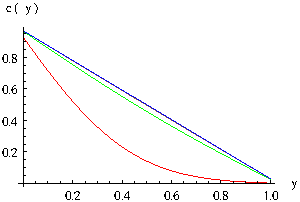
\includegraphics[width=0.33\textwidth]{jacobi32.pdf}}
  \subfloat{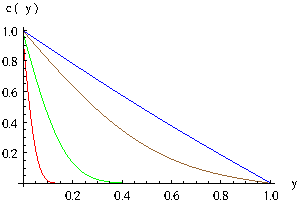
\includegraphics[width=0.33\textwidth]{jacobi256.pdf}}
  \subfloat{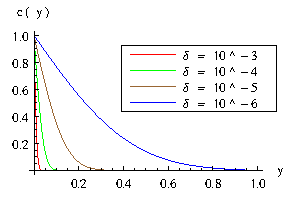
\includegraphics[width=0.33\textwidth]{jacobi1024.pdf}}
  \caption{The quality of the solution at the iteration where the threshold $\delta$ is reached for $N = 32$ (left) , $N = 256$ (middle) and $N = 1024$ (right).}
  \label{fig:jacobi}
\end{figure}

From the table we see that for $\delta = 10^{-3}$ there is no difference between different matrix sizes. However this changes when $\delta$ gets smaller. This has to do with the speed at which the solutions converge to the limit solution (the straight line). If we look at the figures we see that for $N = 32$ for $\delta = 10^{-5}$ and lower the solution is nearly a straight line and so the difference between subsequent iterations will be very small and the threshold is reached relatively fast. However for $N = 256$ and $N = 1024$ the solution is not nearly reached and so it takes much more iterations for the simulation to reach the threshold. Even when looking at the same threshold values we see that the solution is worse for increasing size, even though the number of iterations performed is much larger. Hence the Jacobi iteration is not a very efficient method, since for large matrices (which is what we are usually interested in) it takes a long time to get any kind of reasonable convergence in terms of the analytical solution, not the value of $\delta$.

\subsubsection{Gauss-Seidel iteration}

For the Gauss-Seidel iteration we will do three checks: we will check the correctness of the solution, the convergence of the solution and the scalability of the code.

We start with the correctness of the solution, in figure \ref{fig:gausscorr} below we see the solution for $\delta = 10^{-2}$ (left) $\delta = 10^{-3}$ (middle) and $\delta = 10^{-5}$ (right) for a matrix size of 100. We visualized by combining the data from four processors (to check if the parallel implementation is correct). We see indeed that as $\delta$ decreases (corresponding to an increasing number of iterations) that diffusion takes place. Also we see that the solution is not dependent on the $x$ coordinate which, as argued before, is what we expect with this particular set of initial conditions. Hence we can conclude that our diffusion model is correct.

\begin{figure}[H]
  \centering
  \subfloat{
\includegraphics[width=0.33\textwidth]{gauss02.pdf}}
  \subfloat{
\includegraphics[width=0.33\textwidth]{gauss03.pdf}}
  \subfloat{
\includegraphics[width=0.33\textwidth]{gauss05.pdf}}
  \caption{The solution of cylindrical heat diffusion with convergence threshold $10^{-2}$ (left) $10^{-3}$ (middle) and $10^{-5}$ (right).}
  \label{fig:gausscorr}
\end{figure}

Furthermore we checked after how many iterations a certain convergence threshold is reached. We did this for $N = 32, 256, 1024$ and $\delta = 10^{-3..6}$. The results are given in table \ref{tab:gausscorr} below:

\begin{table}[H]
  \centering
  \begin{tabular}{l | c | c | c}
    \hline
    $\delta$ & $N = 32$ & $N = 256$ & $N = 1024$ \\
    \hline
    $10^{-3}$ & 280 & 300 & 300\\
    $10^{-4}$ & 790 & 2970 & 2970\\
    $10^{-5}$ & 1300 & 23670 & 29840\\
    $10^{-6}$ & 1810 & 54510 & 278740\\
  \end{tabular}
  \caption{The iteration number at which the threshold value $\delta$ is reached for various matrix sizes.}
  \label{tab:gausscorr}
\end{table}

If we compare this table with table \ref{tab:gauss} we see that it generally takes more iterations to reach the same threshold in the case of the Gauss-Seidel iteration compared to the Jacobi iteration. The number of iterations is only smaller when $\delta = 10^{-6}$ and $N = 32$ or 256. This is a strange results since one would intuitively say that it would take less iterations to reach the convergence threshold. However, the convergence threshold does not necessarily have to do much with the convergence to the exact solution of the problem, in this case a straight line. We can show that in the following figure \ref{fig:gauss} below, where we have plotted the solution for the convergence thresholds $\delta = 10^{-3..6}$ for the Gauss-Seidel iteration (so at the iteration values from table \ref{tab:gausscorr} above) and we also plotted the solution at the same convergence thresholds for the Jacobi iteration, which are the same graphs as in figure \ref{fig:jacobi}. We see that while it takes more iterations to reach a certain threshold (usually about 20\% - 30\% more) we do obtain much better solutions when using the Gauss-Seidel iteration instead of the Jacobi iteration. Also when we would go to even lower thresholds it might be that the large matrix size of 1024 needs less iterations in the case of Gauss-Seidel compared to Jacobi, since smaller matrices already show this inverted behavior when $\delta$ becomes smaller. 

\begin{figure}[H]
  \centering
  \subfloat{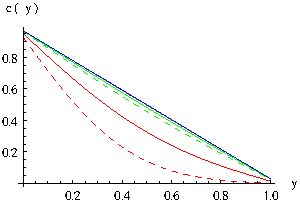
\includegraphics[width=0.33\textwidth]{gauss32.pdf}}
  \subfloat{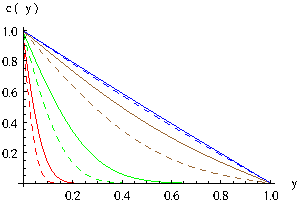
\includegraphics[width=0.33\textwidth]{gauss256.pdf}}
  \subfloat{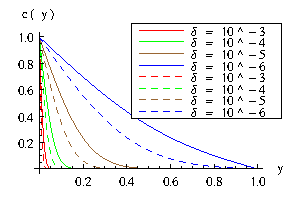
\includegraphics[width=0.33\textwidth]{gauss1024.pdf}}
  \caption{The quality of the solution at the iteration where the threshold $\delta$ is reached for $N = 32$ (left) , $N = 256$ (middle) and $N = 1024$ (right). The dotted lines are the solutions using the Jacobi scheme, the solid lines are the solutions using the Gauss-Seidel scheme.}
  \label{fig:gauss}
\end{figure}

We see that the difference of the quality of the solution increases if the matrix size $N$ increases. Hence for small matrices it is better to use the Jacobi scheme, since the memory usage is not important and the quality of the solution is still good and also the method is faster (presumably, we will check this below). For large matrix sizes however the Gauss-Seidel iteration scheme converges much more to the solution using the same convergence threshold. Although it takes more iterations to get there (20-30\%), the solution is sufficiently closer to the real solution (i.e. the straight line) so that it is still worth wile to implement Gauss-Seidel instead of Jacobi.

Lastly we do a full scalability test, testing for matrix sizes $N = 32..1024$ increasing with a factor 2 and using $p = 1,2,4,8,16$. We set $\delta = 10^{-4}$ such that at least 1000 iterations are performed, regardless of the parameters. We also look at the execution time per iteration for the Jacobi method, to see the difference between the two. The results are given in table \ref{tab:gauss} below:

\begin{table}[H]
  \centering
  \begin{tabular}{l | c | c | c | c | c | c}
    \# Procs & Exec. Time (Jacobi) & Rel. Sp. & Rel. Eff. & Exec. Time (Jacobi) & Rel. Sp. & Rel. Eff.\\
    \hline
    \multicolumn{1}{c}{} & \multicolumn{3}{c}{$N = 32$} & \multicolumn{3}{c}{$N = 64$} \\
    \hline
    1 & 0.000007 (0.000003) & 1 & 1 & 0.000029 (0.000010) & 1 & 1\\ 
    2 & 0.000012 (0.000005) & 0.58 & 0.29 & 0.000024 (0.000007) & 1.21 & 0.60\\
    4 & 0.000016 (0.000009) & 0.44 & 0.11 & 0.000020 (0.000009) & 1.45 & 0.37\\
    8 & 0.000016 (0.000013) & 0.44 & 0.06 & 0.000017 (0.000009) & 1.71 & 0.22\\
    16 & 0.000017 (0.000012) & 0.41 & 0.03 & 0.000017 (0.000010) & 1.71 & 0.11\\
    \hline
    \multicolumn{1}{c}{} & \multicolumn{3}{c}{$N = 128$} & \multicolumn{3}{c}{$N = 256$} \\
    \hline
    1 & 0.000125 (0.000047) & 1 & 1 & 0.000516 (0.000185) & 1 & 1\\
    2 & 0.000073 (0.000026) & 1.71 & 0.86 & 0.000270 (0.000097) & 1.91 & 0.96\\
    4 & 0.000045 (0.000017) & 2.78 & 0.70 & 0.000145 (0.000053) & 3.56 & 0.89\\
    8 & 0.000030 (0.000013) & 4.17 & 0.52 & 0.000082 (0.000031) & 6.29 & 0.78\\
    16 & 0.000023 (0.000012) & 5.43 & 0.34 & 0.000050 (0.000020) & 10.32 & 0.65\\
    \hline
    \multicolumn{1}{c}{} & \multicolumn{3}{c}{$N = 512$} & \multicolumn{3}{c}{$N = 1024$} \\
    \hline
    1 & 0.002087 (0.000770) & 1 & 1 & 0.009297 (0.006712) & 1 & 1\\ 
    2 & 0.001061 (0.000390) & 1.97 & 0.98 & 0.005065 (0.004397) & 1.84 & 0.92\\ 
    4 & 0.000544 (0.000190) & 3.84 & 0.96 & 0.002966 (0.003305) & 3.13 & 0.78\\
    8 & 0.000282 (0.000101) & 7.40 & 0.93 & 0.001894 (0.002849) & 4.91 & 0.62\\
    16 & 0.000152 (0.000055) & 13.73 & 0.86 & 0.001110 (0.002455) & 8.38 & 0.52 \\
  \end{tabular}
  \caption{Execution time (execution time for Jacobi), relative speedup and relative efficiency as a function of grid points and number of processes.}
  \label{tab:gauss}
\end{table}

From the table we find a behavior which is similar to the measurements made in the previous assignment. We find no speedup for small matrix sizes, but the speedup improves for increasing matrix sizes. Note that the maximum speedup achieved is 13.73 for 16 cores with a matrix size of $N = 512$, which is an efficiency of 86\%. For a matrix size of 1024 the performance is less, this has probably to do with the (halve) rows being too large to be send in one piece during the communication. Since the row has to be chopped up in some additional pieces and then send, this takes much more extra time, hence the relatively worse performance when comparing the speedup between $N = 512$ and $N = 1024$. 

As expected, the Jacobi iteration is faster since we can do one iteration as a whole instead of having to use the checkerboard method as with Gauss-Seidel. However, for $N = 1024$ this is not the case and the Jacobi implementation is much slower (more than a factor 2) for a large number of cores. Since the Gauss-Seidel does the same as Jacobi does but even more, the only possible explanation is the use of only one matrix instead of two. This again only plays a role when the matrices are large, because they do not fit in the cache anymore. Since the Jacobi implementation uses only one matrix this saves loading matrix elements from the other matrix. So the use of this matrix, next to saving memory, can have an impact on performance, provided the matrices are large and many cores are used.

In the previous assignment (modeling the non-steady state) we only found a maximum speedup of 5.83 for 16 cores, which is much less than we found here. However, in that case we used three different matrices which gives even more cache slowdown and also the computation of new grid points is slightly more complicated (but these extra floating point operations count heavily since they are in a for loop). The message exchange is nearly the same (with the Gauss-Seidel matrix chopping communication in two pieces) so the difference has to come from the problems with loading of three matrices in the cache.

\subsection{Conclusion}
We have used to code from the previous exercise, heat diffusion on a cylinder, and adjusted it for the steady state. First we implemented a stopping condition and measured the overhead induced by this implementation which is significant and scales with the number of processes. Then we used two methods, Jacobi and Gauss-Seidel iteration to investigate the convergence of the steady state solution. We checked the validity of both models as well as the extra overhead produced, and found a somewhat slower but much better convergence for the Gauss-Seidel iteration. For the Gauss-Seidel iteration we also performed a scalability test and found good speedups for large matrices, better than in the case of the previous assignment, probably because of the use of two less matrices. Jacobi in general outperformed Gauss-Seidel, except for a large number of cores and large matrices, because the Jacobi method uses an extra matrix, which gives slowdown when loading into the cache. 

\end{document}